\chapter{Design}

In this section, the benchmark problem will be defined and mapped as DCOP, the framework design will be explained and the mapping of the algorithms on to the Signal/Collect framework will be described. Additionally, the design and considerations regarding the monitoring platform will be presented.

\section{Meeting Scheduling Problem}

\subsection{Formal Definition as DCOP}

The formulation of the meeting scheduling problem follows the basic definition of a distributed constraint optimization problem. Agents, variables and their relationships, as well as constraints shall be formulated. The components of a meeting scheduling problem are participants, their schedule, meetings and a given timeframe. For the sake of simplicity, it was decided to not take travel time between meetings or other parameters into consideration as certain researchers have done \cite{Grubshtein}. It was also decided to use utilities instead of costs. % FIXME find zitat

\theoremstyle{hardconstraint2}
\newtheorem{hardconstraint2}{Definition}
\begin{hardconstraint2}
Participant - has preferences and meeting he/she need to attend
\end{hardconstraint2}
\begin{hardconstraint2}
Meeting - has participants and needs to be held at an agreable time
\end{hardconstraint2}

%-------------------------- Variable  & Agent definition ------------------------------------------------
\begin{figure}[h!]
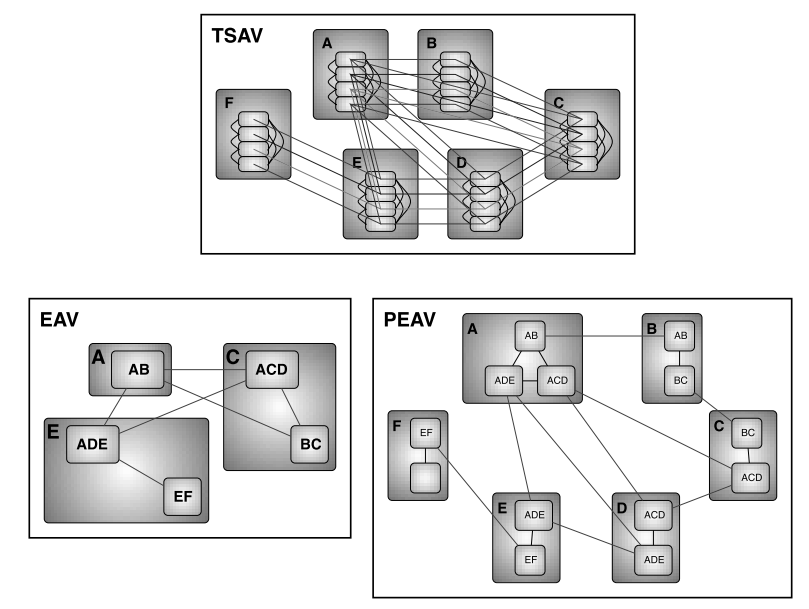
\includegraphics[width=300px]{graphics/variablemodell.png}
\caption{Different paradigms of mapping the meeting scheduling Problem \cite{Maheswarana}.}
\label{fig:variablemapping}
\end{figure}
Maheswarana et al. propose three different ways of mapping a meeting scheduling problem to variables (Figure \ref{fig:variablemapping}). TSAV (Time Slots As Variables), EAV (Event As Variables) and PEAV (Private Events As Variables). In EAV, every participant holds a private variable containing the timeslot that should be used for a meeting. PEAV is a modification of the EAV paradigm where agents don't share their local valuations \cite{Maheswarana,}. It was decided to follow the PEAV principle and model every meeting participation of an agent as one variable instead of using timeslots as variables. An agent therefore can hold multiple variables. This paradigm has also been tried by other researchers, which further established confidence in the decision \cite{Petcu2003}.
\begin{hardconstraint2}
Agent - holds one variable per meeting participation
\end{hardconstraint2}
\begin{hardconstraint2}
Variable - represents one meeting participation
\end{hardconstraint2}
%---------------------------- Domain & Value  definition -----------------------------------------------
A variable takes on a value \(s_{i} \in S_{i}\) in a defined problem domain \(D\). In the formulation of the meeting scheduling problem, the domain represents a finite set of timeslots and the variable assigns to one of these timeslots. This value represents the currently locally chosen timeslot for a specific meeting.
\begin{hardconstraint2}
Domain - holds a finite set of possible timeslots to schedule a meeting
\end{hardconstraint2}
\begin{hardconstraint2}
Value - assigns to a timeslot of the available timeslots in the Domain
\end{hardconstraint2}
%------------------------------ Constraints ---------------------------------------------------
From the problem definition in the background \& related work chapter one can derive soft and hard constraint. Soft constraints can possibly be constructed from the preferences of the participants and utilized to maximize the utility \cite{Franzin}. As the global utility should be optimized, the participants could as a consequence have a low local utility. Three differently weighted soft constraints have been defined to model preferences of agents. Preferred timeslots gain the highest utility, followed by free timeslots and blocked timeslots, which gain no value at all. Further, a timeliness soft constraint was defined that adds a higher utility to earlier timeslots. All of the soft constraints have unary relationships, i.e. are local. % FIXME \cite{Chapman2011} \cite{chun, andy 2003}\cite{mes, martijn 2007}\cite{BenHassine2007}\cite{Berger2008}
Additionally, two hard constraints with k-ary relationships to variable neighbours need to be formulated. The first would be an equality constraint for assigned values for a meeting timeslot between all variables related to a meeting. The second is a difference constraint of assigned values between all variables of an agent \cite{Farinelli, Angulo}.
\newline\newline
So, a local utility function \(u_{l}(s)\) would include the sum of all soft constraints multiplied by the product of the hard constraints analogous to the global function defined in chapter 2.
\[ u_{l}(s) = \prod_{\substack{hc_{k} \in HC}} u_{SC_{g}}(s) \bigg( \sum_{sc_{k} \in SC} u_{SC_{g}}(s) \bigg)\] 


\subsection{Problem Dataset Generation}

% ------------------------ Entscheidung, Verteidigung --------------------
During the course of the thesis, it was necessary to find a dataset for benchmarking. The Frodo2 framework does provide a couple of datasets for meeting scheduling. But because it was considered that in the benchmarks one would need to be able to produce problems with different densities and scale to high numbers of participants, it was decided to generate meeting participations and schedules randomly.

The meeting participations are limited to a maximum of five. BECAUSE

Distributed Meeting Scheduling: CHAPTER 10

\section{Mapping of DPOP}

based on: A Scalable Method for Multiagent Constraint Optimization
breakdown
   
%----------------- Code & Mapping ----------------------

\begin{algorithm}
\caption{DPOP Pseudocode}\label{euclid}
\begin{algorithmic}[1]
\Procedure{MyProcedure}{}
\State $\textit{stringlen} \gets \text{length of }\textit{string}$
\State $i \gets \textit{patlen}$
\BState \emph{top}:
\If {$i > \textit{stringlen}$} \Return false
\EndIf
\State $j \gets \textit{patlen}$
\BState \emph{loop}:
\If {$\textit{string}(i) = \textit{path}(j)$}
\State $j \gets j-1$.
\State $i \gets i-1$.
\State \textbf{goto} \emph{loop}.
\State \textbf{close};
\EndIf
\State $i \gets i+\max(\textit{delta}_1(\textit{string}(i)),\textit{delta}_2(j))$.
\State \textbf{goto} \emph{top}.
\EndProcedure
\end{algorithmic}
\end{algorithm}

\subsection{Graph Structure}


\subsection{Vertices}


\section{Mapping of MGM}

This is the pseudocde for the Maximum-Gain messaging algorithm that has been used to implement \cite{Chapman2011}.

%currentReward5u(s5currentState, sv)1 for k51:K
%2
%stateGain(k)5u(s5k, sv) – currentReward
%3
%end for
%4
%bestGainState5argmax
%½stateGain?
%5
%k
%bestGainValue5stateGain(bestStateGain)
%6
%sendBestGainMessage[allNeighbours, bestGainValue]
%7
%neighbourGainValues5getNeighbourGainValues[allNeighbours]
%8
%if bestGainValue.max[neighbourGain] then
%9
%newState5bestGainState
%10
%sendStateMessage[allNeighbours, newState]
%11
%end if
%12

    \begin{algorithm}
\caption{MGM Pseudocode}\label{euclid}
\begin{algorithmic}[2]
\Procedure{MyProcedure}{}
\State $\textit{stringlen} \gets \text{length of }\textit{string}$
\State $i \gets \textit{patlen}$
\BState \emph{top}:
\If {$i > \textit{stringlen}$} \Return false
\EndIf
\State $j \gets \textit{patlen}$
\BState \emph{loop}:
\If {$\textit{string}(i) = \textit{path}(j)$}
\State $j \gets j-1$.
\State $i \gets i-1$.
\State \textbf{goto} \emph{loop}.
\State \textbf{close};
\EndIf
\State $i \gets i+\max(\textit{delta}_1(\textit{string}(i)),\textit{delta}_2(j))$.
\State \textbf{goto} \emph{top}.
\EndProcedure
\end{algorithmic}
\end{algorithm}

\subsection{Graph Structure}
\subsection{Vertices}

\section{Mapping of MaxSum}

%Aji, S. M. and McEliece, R. J. 2000. The generalized distributive law. IEEE Transactions on Information Theory 46,
    
This is the pseudocode of the MaxSum algorithm that has been used for the implementation \cite{Zivan2012}.

Max-sum (node n)
%1. Nn ←all of n’s neighboring nodes 2. while (no termination condition is met) 3.
%collect messages from Nn
%4.
%for each n? ∈ Nn
%5.
%if (n is a variable-node)
%6.
%produce messagemn? using messages from Nn \ {n?}
%7.
%if (n is a function-node)
%8.
%produce messagemn? using constraint and messages from Nn \ {n?}
%9. sendmn? to n?

    \begin{algorithm}
\caption{Maxsum Pseudocode}\label{euclid}
\begin{algorithmic}[3]
\Procedure{MyProcedure}{}
\State $\textit{stringlen} \gets \text{length of }\textit{string}$
\State $i \gets \textit{patlen}$
\BState \emph{top}:
\If {$i > \textit{stringlen}$} \Return false
\EndIf
\State $j \gets \textit{patlen}$
\BState \emph{loop}:
\If {$\textit{string}(i) = \textit{path}(j)$}
\State $j \gets j-1$.
\State $i \gets i-1$.
\State \textbf{goto} \emph{loop}.
\State \textbf{close};
\EndIf
\State $i \gets i+\max(\textit{delta}_1(\textit{string}(i)),\textit{delta}_2(j))$.
\State \textbf{goto} \emph{top}.
\EndProcedure
\end{algorithmic}
\end{algorithm}

\subsection{Graph Structure}

-- describe tests and thinking behind the chosen structure!!!!

\subsection{Vertices}

\section{Framework}

\subsection{Signal / Collect}

It was decided to build a specific framework for benchmarking dynamic problems. The foundation of the framework is the Signal/Collect framework \cite{Stutz2010}\footnote{http://uzh.github.io/signal-collect}, which is built on top of Akka\footnote{http://akka.io} and written in Scala\footnote{http://www.scala-lang.org}. It is a graph processing engine with a programming model that features vertices and edges. The vertices have a state and send signals along the edges to other vertices, which can contain any datatype. The signal usually is their state or in context of their state. The vertices collect the signals and perform a compution on the collected data, before adjusting their state according to the calculations and sending out the newly generated signal.  This model allows to reduce complex algorithms to a few lines of code and is applicable for many problems. The reason for choosing this framework in this thesis is the structural fit to distributed constraint optimization problems and the possiblity to add and remove vertices during runtime. This allows for dynamically changing problem computations. Further, the capability of running problems asynchronously or with synchronous signal steps and the possibility to distribute the system on multiple machines add to the advantages.

\subsection{Parameters \& Modes}
This framework was designed with the benchmarks in mind.  It should be possible to pass the general run parameters like which algorithm to use, which Signal/Collect run mode (synchronous/asynchronous) to use, normal run mode or dynamic variations (changeConstraints, changeVariable, changeDomain) with specific parameters. For testing, two test modes were implemented: SingleTest and MultiTest. Single Test is for single runs obviously and MultiTest allows to specifiy how many runs each specification should be doing to create a median of those runs, how much the agents respectively the meetings should increase after a specification has been processed and where to stop. By this, it is possible to explore an area of specifications. Finally, it should be possible to define different problems. For this thesis, the parameters for problem density (blocked timeslots percentage), timeslots, meetings and agents were defined.

\subsection{Functionality \& Structure}

The considerations for the structure were that I needs to be hierarchical to allow different constraint optimization problems to be run on the framework. So, the hierachy goes from a Base to a Dynamic to a Problem level. It should include ProblemFactories and Problems, GraphFactories and Graphs, as well as Vertices.\newline\newline

- Problem Factory: Problem -> MeetingSchedulingProblem class diagram

- Graph Factory: Graph -> DPOP Graph, MGM Graph, MaxSum Graph explanation 
- Graph

- BasicVertex -> DynamicVertex -> MeetingSchedulingVertex -> DPOP, MGM, MaxSum Vertex class diagram!!!

\subsection{Dynamics Controller}

how does it work, what can it do

- Registration of vertices
- change constraints
- change variables
- change domain

- Initial design consideration was to make it part of the graph as signal collect allows mixup of different types. Created weird problems because I need to pause the vertex for interval changes. not part of the graph but connected to vertices -> because it was a problem with convergence and there was a problem with thread sleep in akka

\section{Monitoring Platform}

It was decided to find a more sophisticated method to monitor the utility, quality, conflicts and stats of the calculations than to write to a logfile. Partially because File IO can possibiliy be limited in the number of open files and processing results to fit the log file format during calculations can affect the performance of the algorithm one tries to benchmark. Mainly because processing log files was to tedious and visibility was not given to the calculations.

Sending the results with non-blockin http requests to a restful server was considered to be an alternative and the Play Framework\footnote{https://www.playframework.com} has been chosen because it is highly scalable, is able to handle thousands of simultanous connections, lightweight, non-blocking and allows to process results on-the-fly with code in Java or Scala. It was also chosen because Akka is tightly integrated and the actors concept are an integral part of the framework. It further allows to preview the calculation of the graph in realtime with websockets, which can be helpful during the implementation of algorithms.

By using an actor based approach it is possible to contain run specific data in a closed entity and store when limits are reached. Through the chosen architecture one can run multiple tests in parallel without problems. The server is of course also limited by it's ressources.

For asynchronous http request the Dispatch\footnote{http://dispatch.databinder.net} library has been used.

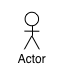
\includegraphics{graphics/monitoring}


